\documentclass{article}
%\usepackage[citestyle=authortitle-terse,backref]{biblatex}
%\addbibresource{homotopy-theory.bib}

\usepackage[left=4cm, right=4cm]{geometry}
\usepackage{palatino,eulervm,dutchcal,xcolor}
\usepackage{graphicx,subcaption,float}
\usepackage{enumitem,parskip,multicol,array}
\newcolumntype{L}{>{$}c<{$}}%table in mathmode
\usepackage{amsthm,amssymb,amsmath,mathtools,thmtools,tikz,tikz-cd}
\usetikzlibrary{%
	matrix,%
	calc,%
	arrows,%
	shapes,
	decorations.markings,backgrounds,calc,intersections}
\tikzcdset{scale cd/.style={every label/.append style={scale=#1},
		cells={nodes={scale=#1}}}}
\usepackage[bookmarks,bookmarksopen,bookmarksdepth=3]{hyperref}
\hypersetup{%colores
	colorlinks=true,
	urlcolor=blue,
	linkcolor=magenta,
	citecolor=blue,
	filecolor=blue,
	urlbordercolor=white,
	linkbordercolor=white,
	citebordercolor=white,
	filebordercolor=white}
\usepackage{cleveref}

\definecolor{blue-violet}{rgb}{0.54, 0.17, 0.89}
\definecolor{azure}{rgb}{0.0, 0.5, 1.0}
\definecolor{green(ncs)}{rgb}{0.0, 0.62, 0.42}
\definecolor{forestgreen}{rgb}{0.13, 0.55, 0.13}
\definecolor{limegreen}{rgb}{0.2, 0.8, 0.2}
\definecolor{palatinateblue}{rgb}{0.15, 0.23, 0.89}
\definecolor{trueblue}{rgb}{0.0, 0.45, 0.81}
\definecolor{goldenyellow}{rgb}{1.0, 0.87, 0.0}
\definecolor{fashionfuchsia}{rgb}{0.96, 0.0, 0.63}
\definecolor{brightcerulean}{rgb}{0.11, 0.67, 0.84}
\definecolor{jonquil}{rgb}{0.98, 0.85, 0.37}
\definecolor{lavendermagenta}{rgb}{0.93, 0.51, 0.93}
\definecolor{peru}{rgb}{0.8, 0.52, 0.25}
\definecolor{persimmon}{rgb}{0.93, 0.35, 0.0}
\definecolor{persianred}{rgb}{0.8, 0.2, 0.2}
\definecolor{persianblue}{rgb}{0.11, 0.22, 0.73}
\definecolor{persiangreen}{rgb}{0.0, 0.65, 0.58}
\definecolor{persianyellow}{rgb}{0.9, 0.89, 0.0}

\declaretheoremstyle[headfont=\color{trueblue}\normalfont\bfseries,]{colored1}
\declaretheoremstyle[headfont=\color{forestgreen}\normalfont\bfseries,]{colored2}
\declaretheoremstyle[headfont=\color{peru}\normalfont\bfseries,]{colored3}
\declaretheoremstyle[headfont=\color{persiangreen}\normalfont\bfseries,]{colored4}
\declaretheoremstyle[headfont=\color{brightcerulean}\normalfont\bfseries,]{colored5}
\declaretheoremstyle[headfont=\color{lavendermagenta}\normalfont\bfseries,]{colored6}
\declaretheoremstyle[headfont=\color{blue-violet}\normalfont\bfseries,]{colored7}
\declaretheoremstyle[headfont=\color{green(ncs)}\normalfont\bfseries,]{colored8}
\declaretheoremstyle[headfont=\color{peru}\normalfont\bfseries,]{colored9}
\declaretheoremstyle[headfont=\color{persiangreen}\normalfont\bfseries,]{colored10}

\declaretheorem[style=colored1,name=Theorem]{thm}
\declaretheorem[style=colored2,numberlike=thm,name=proposition]{prop}
\declaretheorem[style=colored3,numberlike=thm,name=lemma]{lemma}
\declaretheorem[style=colored4,numberlike=thm,name=corollary]{coro}
\declaretheorem[style=colored5,numbered=no,name=example]{example}
\declaretheorem[style=colored5,numbered=no,name=examples]{examples}
\declaretheorem[style=colored6,numbered=no,name=exercise]{exercise}
\declaretheorem[style=colored7,numbered=no,name=remark]{remark}
\declaretheorem[style=colored8,numbered=no,name=claim]{claim}
\declaretheorem[style=colored9,numbered=no,name=definition]{defn}
\declaretheorem[style=colored10,numbered=no,name=question]{question}

\newcommand{\A}{\mathbb{A}}
\newcommand{\C}{\mathbb{C}}
\newcommand{\D}{\mathbb{D}}
\renewcommand{\H}{\mathbb{H}}
\newcommand{\N}{\mathbb{N}}
\renewcommand{\P}{\mathbb{P}}
\newcommand{\Q}{\mathbb{Q}}
\newcommand{\R}{\mathbb{R}}
\newcommand{\Z}{\mathbb{Z}}

\newcommand{\Ac}{\mathcal{A}}
\newcommand{\Bc}{\mathcal{B}}
\newcommand{\Cc}{\mathcal{C}}
\newcommand{\Dc}{\mathcal{D}}
\newcommand{\Ec}{\mathcal{E}}
\newcommand{\Fc}{\mathcal{F}}
\newcommand{\Gc}{\mathcal{G}}
\newcommand{\Hc}{\mathcal{H}}
\newcommand{\Ic}{\mathcal{I}}
\newcommand{\Jc}{\mathcal{J}}
\newcommand{\Kc}{\mathcal{K}}
\newcommand{\Lc}{\mathcal{L}}
\newcommand{\Mc}{\mathcal{M}}
\newcommand{\Nc}{\mathcal{N}}
\newcommand{\Oc}{\mathcal{O}}
\newcommand{\Pc}{\mathcal{P}}
\newcommand{\Qc}{\mathcal{Q}}
\newcommand{\Rc}{\mathcal{R}}
\newcommand{\Sc}{\mathcal{S}}
\newcommand{\Tc}{\mathcal{T}}
\newcommand{\Uc}{\mathcal{U}}
\newcommand{\Vc}{\mathcal{V}}
\newcommand{\Wc}{\mathcal{W}}
\newcommand{\Xc}{\mathcal{X}}
\newcommand{\Yc}{\mathcal{Y}}
\newcommand{\Zc}{\mathcal{Z}}

\DeclareMathOperator{\Obj}{Obj}
\DeclareMathOperator{\Sing}{Sing}
\DeclareMathOperator{\img}{img}
\DeclareMathOperator{\Ho}{Ho}
\DeclareMathOperator{\Arg}{Arg}
\DeclareMathOperator{\id}{id}
\DeclareMathOperator{\pt}{pt}
\DeclareMathOperator{\Alt}{Alt}
\DeclareMathOperator{\sgn}{sgn}
\DeclareMathOperator{\hTop}{h-Top}
\DeclareMathOperator{\Loc}{Loc}
\DeclareMathOperator{\supp}{supp}
\DeclareMathOperator{\Int}{Int}
\DeclareMathOperator{\Ob}{Ob}
\DeclareMathOperator{\Mor}{Mor}
\DeclareMathOperator{\Cat}{Cat}
\DeclareMathOperator{\Ext}{Ext}
\DeclareMathOperator{\Tor}{Tor}
\DeclareMathOperator{\Top}{Top}
\DeclareMathOperator{\Path}{Path}
\DeclareMathOperator{\Set}{Set}
\DeclareMathOperator{\CGWH}{CGWH}
\DeclareMathOperator{\Hom}{Hom}
\DeclareMathOperator{\Map}{Map}
\DeclareMathOperator{\Tot}{Tot}
\DeclareMathOperator{\K}{K}
\DeclareMathOperator{\CW}{CW}
\DeclareMathOperator{\op}{op}
\DeclareMathOperator{\ev}{ev}
\DeclareMathOperator{\hofib}{hofib}
\DeclareMathOperator{\cofib}{cofib}
\DeclareMathOperator{\hocofib}{hocofib}
\DeclareMathOperator{\rel}{rel}
\DeclareMathOperator{\coker}{coker}
\DeclareMathOperator{\Arr}{Arr}
\DeclareMathOperator{\Funct}{Funct}
\DeclareMathOperator{\gr}{gr}
\DeclareMathOperator{\eq}{eq}
\DeclareMathOperator{\coeq}{coeq}
\DeclareMathOperator{\Cyl}{Cyl}
\DeclareMathOperator{\colim}{colim}
\DeclareMathOperator{\Psh}{Psh}
\DeclareMathOperator{\Sets}{Sets}
\DeclareMathOperator{\Nat}{Nat}
\DeclareMathOperator{\Sh}{Sh}
\DeclareMathOperator{\el}{el}
\DeclareMathOperator{\Spc}{Spc}
\DeclareMathOperator{\Iso}{Iso}
\DeclareMathOperator{\GL}{GL}
\DeclareMathOperator{\SL}{SL}
\DeclareMathOperator{\SO}{SO}
\DeclareMathOperator{\U}{U}
\DeclareMathOperator{\SU}{SU}
\DeclareMathOperator{\Sp}{Sp}
\DeclareMathOperator{\M}{M}
\DeclareMathOperator{\Aut}{Aut}
\DeclareMathOperator{\PGL}{PGL}
\DeclareMathOperator{\PSL}{PSL}
\DeclareMathOperator{\Fun}{Fun}
\DeclareMathOperator{\sSet}{sSet}

\begin{document}
{\Huge higher categories}
%\tableofcontents
\section{18 may}
\subsection{Altan}
\textbf{Plan}
\begin{itemize}
	\item Define Kan complexes, weak kan complexes, homotopy category.
	\item Prove \begin{tikzcd}
		1\text{-cat}\arrow[r,shift={(0,0.05)},"N"]&\arrow[l,shift={(0,-0.05)},"h"]\infty\text{-cat}
	\end{tikzcd}
\end{itemize}
Remember that \textbf{\textit{simplicial sets}} are $\sSet=\Fun(\Delta^{\op},\Set)$. Objects in the category $\Delta$ are lists of numbers $[n]$ and morphisms are nondecreasing maps.
\begin{claim}
	Any morphism in $\Delta$ factors as a product of elements of the following two kinds:
	\[\begin{matrix}
		i_k&&d_k\\
		[n]\to[n+1]&&[n]\to[n-1]\\\\
		0\mapsto 0&&0\mapsto0\\
		1\mapsto1&&1\mapsto1\\
		\cdots&&\cdots\\
		k-1\mapsto k-1&&\\
		k\mapsto k-1&&k\mapsto k\\
		k+1\mapsto k+1&&k+1\mapsto k\\
		&&k+2\mapsto k+1\\
		\cdots&&\cdots\\
		n\mapsto n&&n\mapsto n-1
	\end{matrix}\]
\end{claim}
\begin{remark}
	We can interpret a simplicial set as a sort of simplicial complex by defining $X_n:=X([n])$. In virtue of the claim, knowing all the $X_n$ will not only provide the information where to maps object from $\Delta^{\op}$ to $\Set$, but also where to map morphisms, thus producing a functor in $\Fun(\Delta^{\op},\Set)=\sSet$.
\end{remark}
\begin{remark}For all $k$,
	\[\begin{tikzcd}
		\Sing(X)_n\arrow[r,"d_k",shift={(0,0.06)}]&\Sing(X)_{n+1}\arrow[l,shift={(0,-0.06)},"i_k"]
	\end{tikzcd}\]
	which makes it possible to extend horns to simplices, making $\Sing(X)$ into a Kan complex.
\end{remark}
\begin{defn}[1.1.37, Horn]
	It looks like the horn $\Lambda^n_j$ is just the $n$-simplex after taking away the facet opposite to the $j$-th vertex.
\end{defn}
\begin{remark}
	We did not see definition of spine.
\end{remark}
\begin{defn}[1.1.46, Kan complex]
	If you have a horn in a simplicial set, you can extend it to the simplex, i.e. any lifting problem
	\[\begin{tikzcd}
		\Lambda^n_j\arrow[r]\arrow[d]&X\\
		\Delta^n\arrow[ur,dashed]
	\end{tikzcd}\]
	And a \textbf{\textit{weak Kan complex}} is if for all $0<i<n$ we have \begin{tikzcd}
		D^{n-1}\arrow[r,hook]&D^n=D^{n-1}\times I
	\end{tikzcd}
\end{defn}
\begin{defn}
	Nerve of a category $\Cc$ is the simplicial set given by $[n]\mapsto\Fun([n],\Cc)$. {\color{cyan} So its like a CW complex constructed somehow from another CW complex.}
\end{defn}

\begin{claim}
	$N(\Cc)$ is a weak Kan complex.
\end{claim}
\begin{defn}
	Let $X$ be a weak Kan complex. Define
	\[\Ob X=X([0])\qquad\qquad\Mor X=X([1])\qquad\qquad \Mor(A,B)\ni f\sim g \iff \begin{tikzcd}[row sep=tiny]
	&B\arrow[dd,"\id_B"]\\
	A\arrow[rd,"g",swap]\arrow[ur,"f"]\\
	&B
	\end{tikzcd}\]
\end{defn}
\begin{claim}
	$\sim$ is an equivalence relation.
\end{claim}
\begin{claim}
	$f\sim g$ iff $f^{\op}\sim g^{\op}$ in $X^{\op}$.
\end{claim}
\begin{defn}
	Let $X$ be a weak Kan complex. Then the \textbf{\textit{homotopy category}} $h(X)$ is a category given by
	\[\Ob hX=X([0])\qquad\qquad \Mor hX\text{ are (?) }X([1])/\sim.\]
\end{defn}
\begin{claim}
	\begin{tikzcd}
		1\text{-cat}\arrow[r,shift={(0,0.05)},"N"]&\arrow[l,shift={(0,-0.05)},"h"]\infty\text{-cat}
	\end{tikzcd}
\end{claim}
\subsection{Sergey}
Suppose we have a category $\Cc$ and a simplicial set $X$.
\begin{question}
	What $f:X\to N(\Cc)$ is determined by?
\end{question}
\begin{align*}
	f_0:X_0\to N(\Cc)_0&=\Obj_{\Cc}\\
f_1:X_1\to N(\Cc)_1&=\Hom_{\Cc}\\
f_n:X_n\to N(\Cc)_n&=\left\{\begin{tikzcd}[column sep=tiny,ampersand replacement=\&]
	\bullet\arrow[r,"h_1",no head]\&\bullet\arrow[r,no head]\&\cdots\arrow[r,no head]\&\bullet\arrow[r,"h_n",no head]\&\bullet
\end{tikzcd}\right\}\\
x&\mapsto\begin{tikzcd}[column sep=tiny,ampersand replacement=\&]
	\bullet\arrow[r,"f_1(g^*_0x)",no head]\&\bullet\arrow[r,no head]\&\cdots\arrow[r,no head]\&\bullet\arrow[r,"f_n(g^*_nx)",no head]\&\bullet
\end{tikzcd}
\end{align*}

\section{23 may}
Let's make a dictionary.
\begin{itemize}
	\item Review basic concepts of categories and compare to the world of $\infty$-categories.
\end{itemize}
\[\begin{tikzcd}[row sep=tiny]
	\leavevmode\arrow[r,"N"]&\leavevmode\\
	\leavevmode&\arrow[l,"h",swap]\leavevmode
\end{tikzcd}\]
\begin{tabular}{|p{8cm}|c|}
	\hline
	\textbf{Categories}&\textbf{$\infty$-categories}\\
	\hline\hline
	Category&$\infty$-category/Weak Kan complex \\&($X\in\sSet$ such that $\forall n$ and $\forall 0<i<n$
	
	\\&\begin{tikzcd}
		\Lambda^n_i\arrow[d,hook]\arrow[r,"\forall"]&X\\\Delta^n\arrow[ur,"\exists",dashed]
	\end{tikzcd}).\\\hline

	$\operatorname{\mathcal{G}rp}$, category of grupoids (a groupoid is a category with invertible morphisms)&$\operatorname{Spc}$-$\infty$-category of spaces\\\hline
	$\operatorname{Cat}$, the category of categories & 1-Cat\\\hline
	\hline
\end{tabular}
\begin{defn}
	A \textbf{\textit{grupoid}} is a category where every morphism is invertible.
\end{defn}
\begin{example}\leavevmode
	\begin{itemize}
		\item A grupoid with only one object is a group since the automorphism set of the object is a group.
		\item Let $X\in\Top$. The \textbf{\textit{fundamental grupoid $\Pi_1(X)$}} is the grupoid whose objects are points of $X$ and morphisms paths modulo homotopy.
		\item $\Sing(X)\in\sSet$ where $\Sing(X)_n=\Hom_{\Top}(|\Delta^n|,X)$.
		\begin{claim}
			$\Sing(X)$ is a Kan complex.
		\end{claim}
	\end{itemize}
\end{example}
\begin{defn}
	The \textbf{\textit{nerve of a category $\Cc$}} is $N(\Cc)_n=\Fun([n],\Cc)=\{(f_0,\ldots,f_n):f_i\in\Cc\text{ composable}\}$.
\end{defn}
\begin{claim}
	$N(\Cc)$ is an $\infty$-category.
\end{claim}
\begin{proof}
	Obvious (compose morphism).
\end{proof}
\begin{defn}
	Given $\Cc\in\infty-\Cat$, its \textbf{\textit{homotopy category}} $h(\Cc)$ is a 1-Category whose objects are $C_0:=\Cc([0])$ and morphisms are $\Cc_1/\sim$ where $\sim$ means that two parallel morphisms $f,g:a\to b$ are \textbf{\textit{homotopic}} if, when thinking about $f,g$ as edges of a simplicial complex, there exists a 2-face inside the triangle given by $f,g,\id_b$ {\color{red}yes}.
\end{defn}
\begin{lemma}
	$f\sim g$ and $f\sim h$ implies $g\sim h$.
\end{lemma}
\begin{proof}
	\[\begin{tikzcd}
		\bullet&\bullet\arrow[l,"\id",swap]\arrow[r,"\id"]&\bullet\arrow[ll, bend right,dashed,swap,"\exists"]\\
		&\bullet\arrow[ul,"h"]\arrow[u,"f"]\arrow[ur,"g",swap]
	\end{tikzcd}\]
	and it does exists because, if you look well, there is a horn:
	\begin{center}
		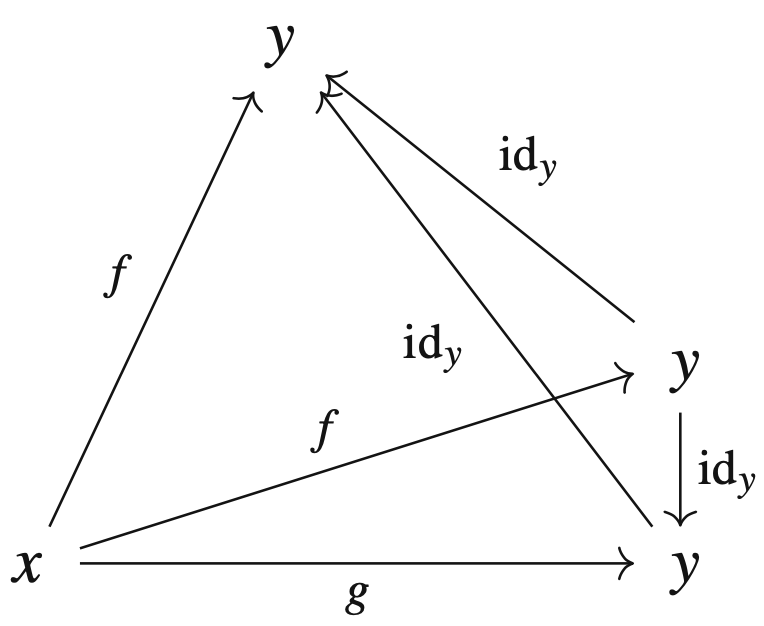
\includegraphics[width=0.3\linewidth]{dgm1}
	\end{center}
\end{proof}
The objective of this talk actually was to compare some usual objects in category theory to their analogues in $\infty$-categories. So recall
\begin{remark}\leavevmode
	\begin{itemize}
		\item The category of categories is a category.
		\item The functors between to categories form a category.
		\item \begin{thm}
			$\Fc\to\Gc$ is an equivalent iff it is fully faithful and essentially surjective.
		\end{thm}
		\item $\Mor_{\Cc}(X,Y)$ is a set and $\Cc$ are enriched over $\Set$.
	\end{itemize}
\end{remark}
\begin{prop}
	A 1-category enriched over $\Spc$ iff it is an $\infty$-category.
\end{prop}
\begin{example}
	$h(\Sing(X))$ is just the fundamental grupoid.
\end{example}

\section{June 15}\label{sec:June 15}


%\addcontentsline{toc}{section}{References}
%\printbibliography
\end{document}
